\section{Introduction}

\ifdefined\DEBUG \todo[inline]{Why is the subject/problem area important?} \else \fi
\textit{Wireless sensor networks (WSNs)} have many environmental monitoring applications and on-going research in areas such as oceanographic measurement \citep{Mahdy2008a, Albaladejo2010, 6973877}, radioactive contamination \citep{Gomez2015}, water quality \citep{Fang2010}, flood levels \citep{Castillo-effen2004}, volcanic activity \citep{Werner-Allen2006}, agricultural soil \citep{8745854}, as well as in military uses \citep{6268958}. More recently, the availability and lower cost of low-power wireless transmitters \citep{902661}, solar-harvesting components \citep{Prauzek2018}, and micro-electro-mechanical systems \citep{1045391} has allowed large deployment sizes and scope of use, expanding their real-world use and opening up new areas for practical research \citep{5597912, Kandris2020}.

\ifdefined\DEBUG \todo[inline]{What are the current solutions, what are the problems and how are we improving them?} \else \fi
\ifdefined\DEBUG \todo[inline]{Whats wrong with centralised approaches?} \else \fi
WSNs can be structured with centralised or decentralised control. With centralisation, the controller node has system-wide knowledge, and so allocates measurement tasks to other nodes, orchestrates their communications, and handles recovery (see Figure \ref{fig:wsn_centralised}). This approach inherently does not scale to large networks due to congestion and resource exhaustion on the central component. In harsh environments, this centralisation of control is not robust to damage or node loss. Although there can be learning added to these systems to help optimise in complex systems, non-distributed learning algorithms suffer from the same limitations as non-learning WSN systems \citep{Imagestate2006}. For these reasons, we focus on decentralised, autonomous methods for WSN construction.

\ifdefined\DEBUG \todo[inline]{Whats wrong with decentralised approaches?} \else \fi
With decentralised WSNs, nodes have limited knowledge of the system. Each node acts autonomously to some degree to orchestrate the functionality mentioned above. They are often organised into groups to decrease the cost of coordination without full centralisation. The basis of many of these decentralised techniques is hierarchical, typically some form of clustering technique. Nodes are formed into sub-groups with designated leaders that orchestrate the behaviours of each group of nodes and communicates with the central controller (see Figure \ref{fig:wsn_clustering}) . This ability for nodes to work autonomously increases resilience but introduces new challenges. In working with local information only, the system can fail to optimise well or get trapped in local optima. In addition, system-wide coordination of node behaviours is difficult when communication is limited to small sets of neighbours \citep{Carlos-Mancilla2016}.
\begin{figure}
	\begin{subfigure}{0.5\textwidth}
		\centering
		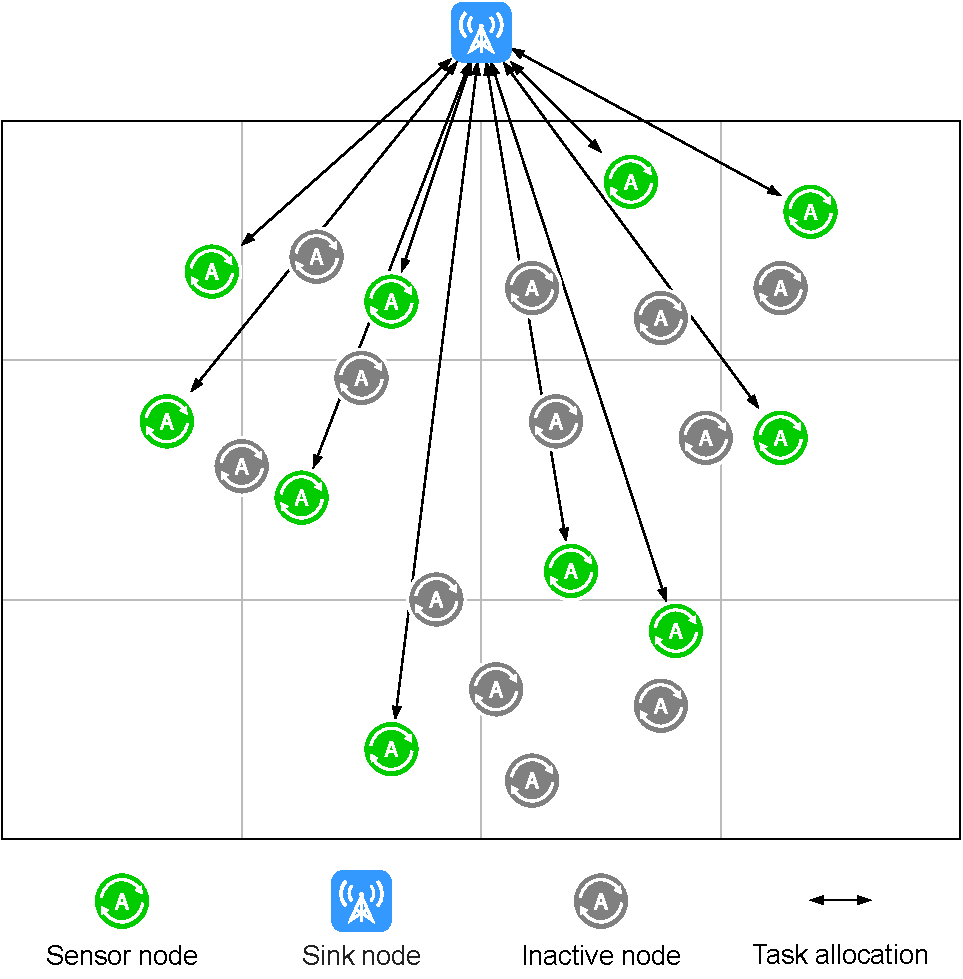
\includegraphics[width=.8\linewidth]{WSN_centralised}
		\caption{A centralised WSN configuration with direct communication}
		\label{fig:wsn_centralised}
	\end{subfigure}%
	\begin{subfigure}{0.5\textwidth}
		\centering
		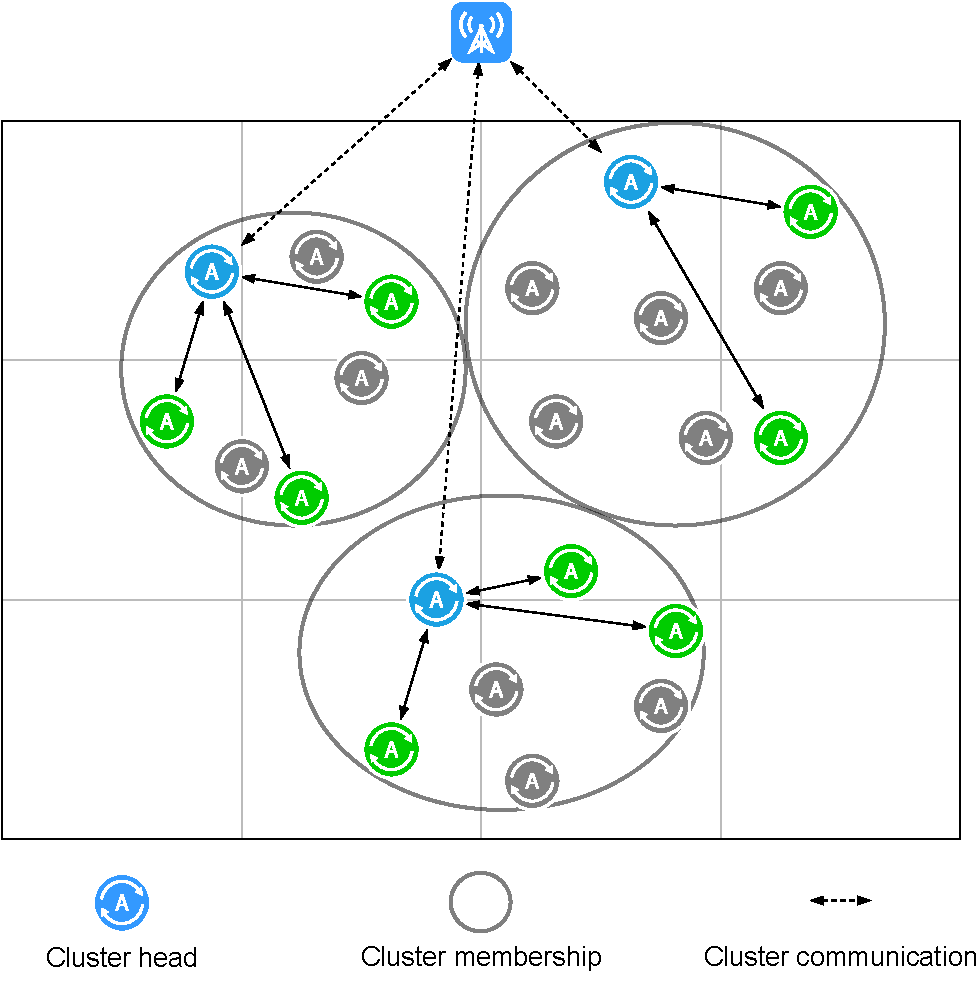
\includegraphics[width=.8\linewidth]{WSN_clustering}
		\caption{A decentralised WSN configuration based on clustering}
		\label{fig:wsn_clustering}
	\end{subfigure}
	\caption{Common WSN configurations for task coverage of a grid}
	\label{fig:wsn_centralised_decentralised}
\end{figure}

\ifdefined\DEBUG \todo[inline]{Whats wrong with learning approaches?} \else \fi
Reinforcement learning has seen applications in these decentralised systems, often focussed on using adaptive routing  to optimise energy efficiency and system lifetime \citep{ 10.1504/IJCNDS.2012.048871, Kulkarnib}, or to ensure sensor coverage is maintained with the loss of nodes over time \citep{Sharma2020}. These solutions look at single or complementary objective optimisation, and do not take account of the conflicting multiple objectives in WSN systems. System goals may involve energy optimisation, coverage, measurement quality, and how nodes allocate resources to meet these goals. The work we present tackles the optimisation of multiple, competing objectives in a WSN system. It also continuously adapts network routes to not only optimise for energy, but also in response to task quality and network impacts.

\ifdefined\DEBUG \todo[inline]{What is the solution and contributions we present?} \else \fi
The solution we present here is based on the following algorithms previously developed by the authors. We use the \acronymATARIA{}{} algorithm to optimise the task of measurements and coverage, minimise the energy consumption of the network, while adapting to the dynamic nature of WSNs \citep{creech2021dynamic}. Through the \acronymMGRAO{}{} algorithm we enable sensors that are taking measurements to optimise the allocation of their resources to meet the overall system goal \citep{creech2021resource}. By combining and evaluating these algorithms in a simulated WSN deployed in a realistic environment, we show that the overall solution can be successfully utilised to balance the systems' multiple objectives of minimising energy consumption, maximising system lifetime, and optimising the quality of the measurement tasks while still maintaining geographical coverage.

\ifdefined\DEBUG \todo[inline]{Structure of paper} \else \fi
In Section \ref{section:background} we look at related research in this area, allowing us to concretely define the problem in Section \ref{section:problem}. Section \ref{section:solution} sets out our solution, followed by definition of the simulated environment and evaluation of the solution in Section \ref{section:experimental}. We close with the summary of our conclusions and future work in Section \ref{section:conclusions}.
